\title{Supplemental figures: Tissue-specific transcriptional patterns underlie seasonal phenotypes in honey bees (\textit{Apis mellifera})}
\author{Sean T. Bresnahan, Mehmet A. Döke, Tugrul Giray, and \\ Christina M. Grozinger}
\date{}

\documentclass[12pt]{article}

\usepackage{graphicx}
\usepackage{subcaption}
\usepackage{longtable}
\usepackage{afterpage} 
\usepackage{caption}
\captionsetup[table]{name=}
\usepackage[nohead, nomarginpar, margin=1in, foot=.25in]{geometry}

\begin{document}
\maketitle

\pagebreak

\begin{figure}[ht]
    \centering
		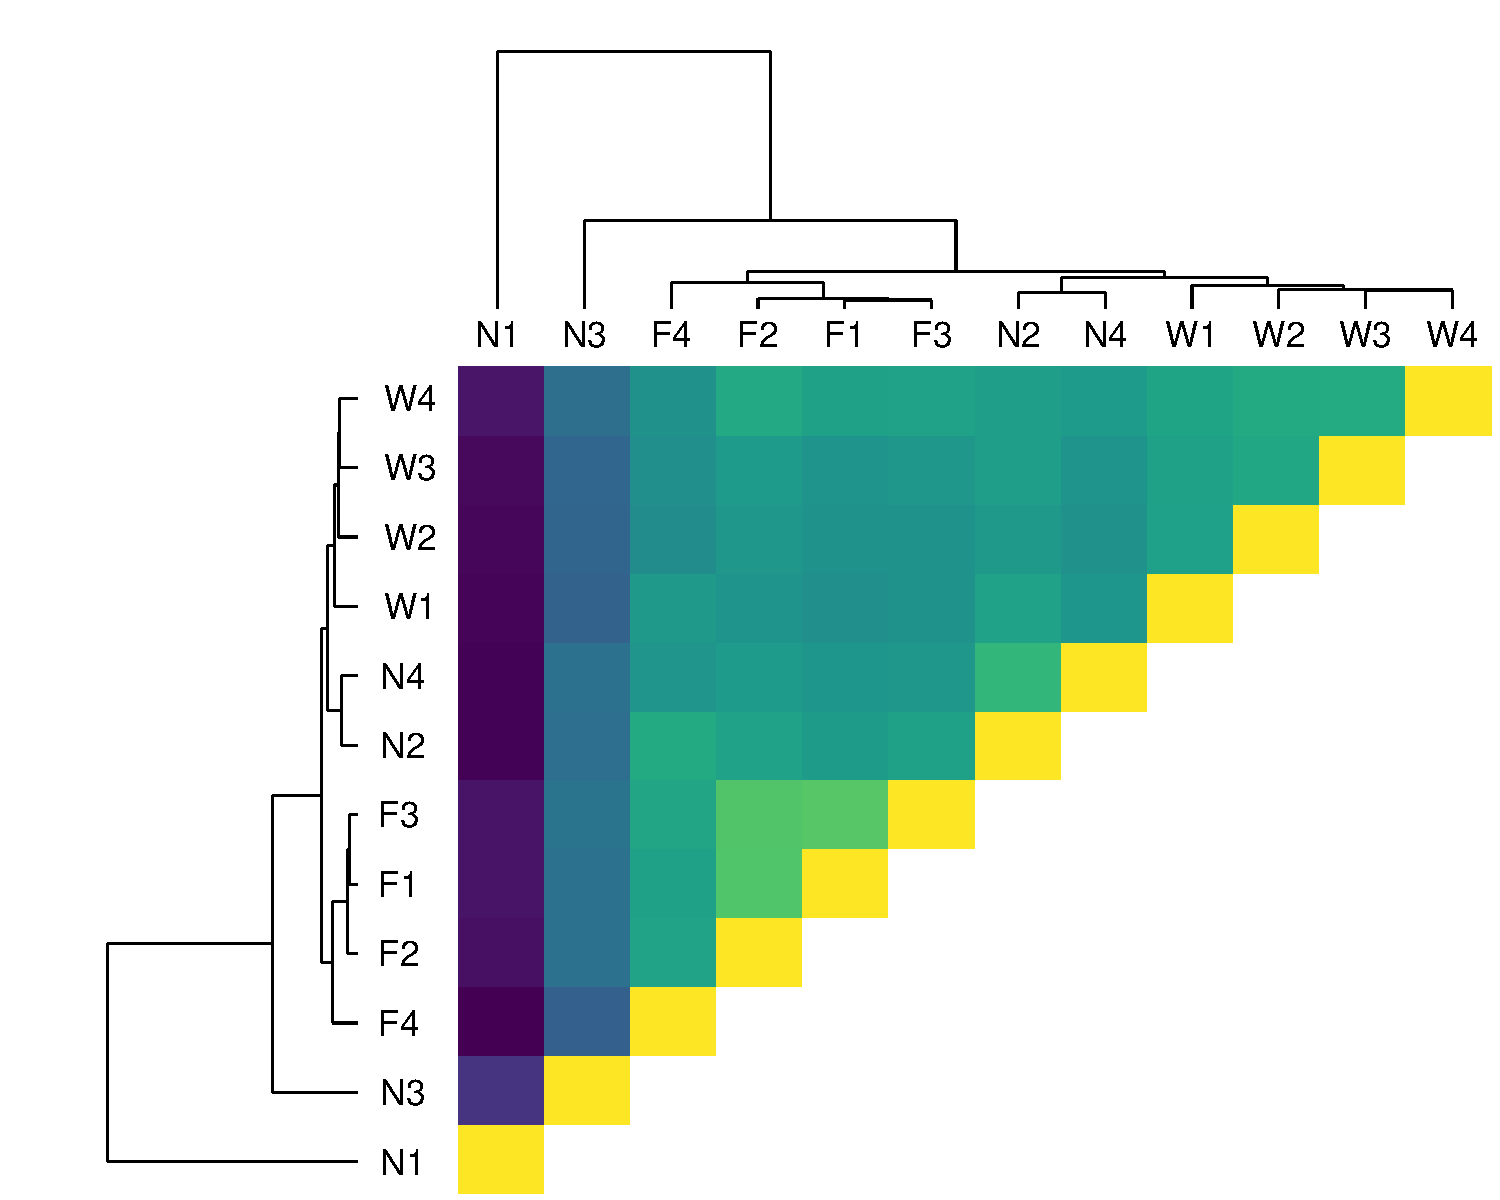
\includegraphics[width=0.75\linewidth]{figs1.pdf} 
    \caption*{\textbf{Figure S1} \quad Fat body tissue sample relationships between nurse, forager, and winter bees as determined by pairwise correlations and hierarchical clustering. Sample relationships determined using all tested genes ($n=9178$).}
    \label{fig:S1}
\end{figure}

\pagebreak

\begin{figure}[ht]
    \centering
		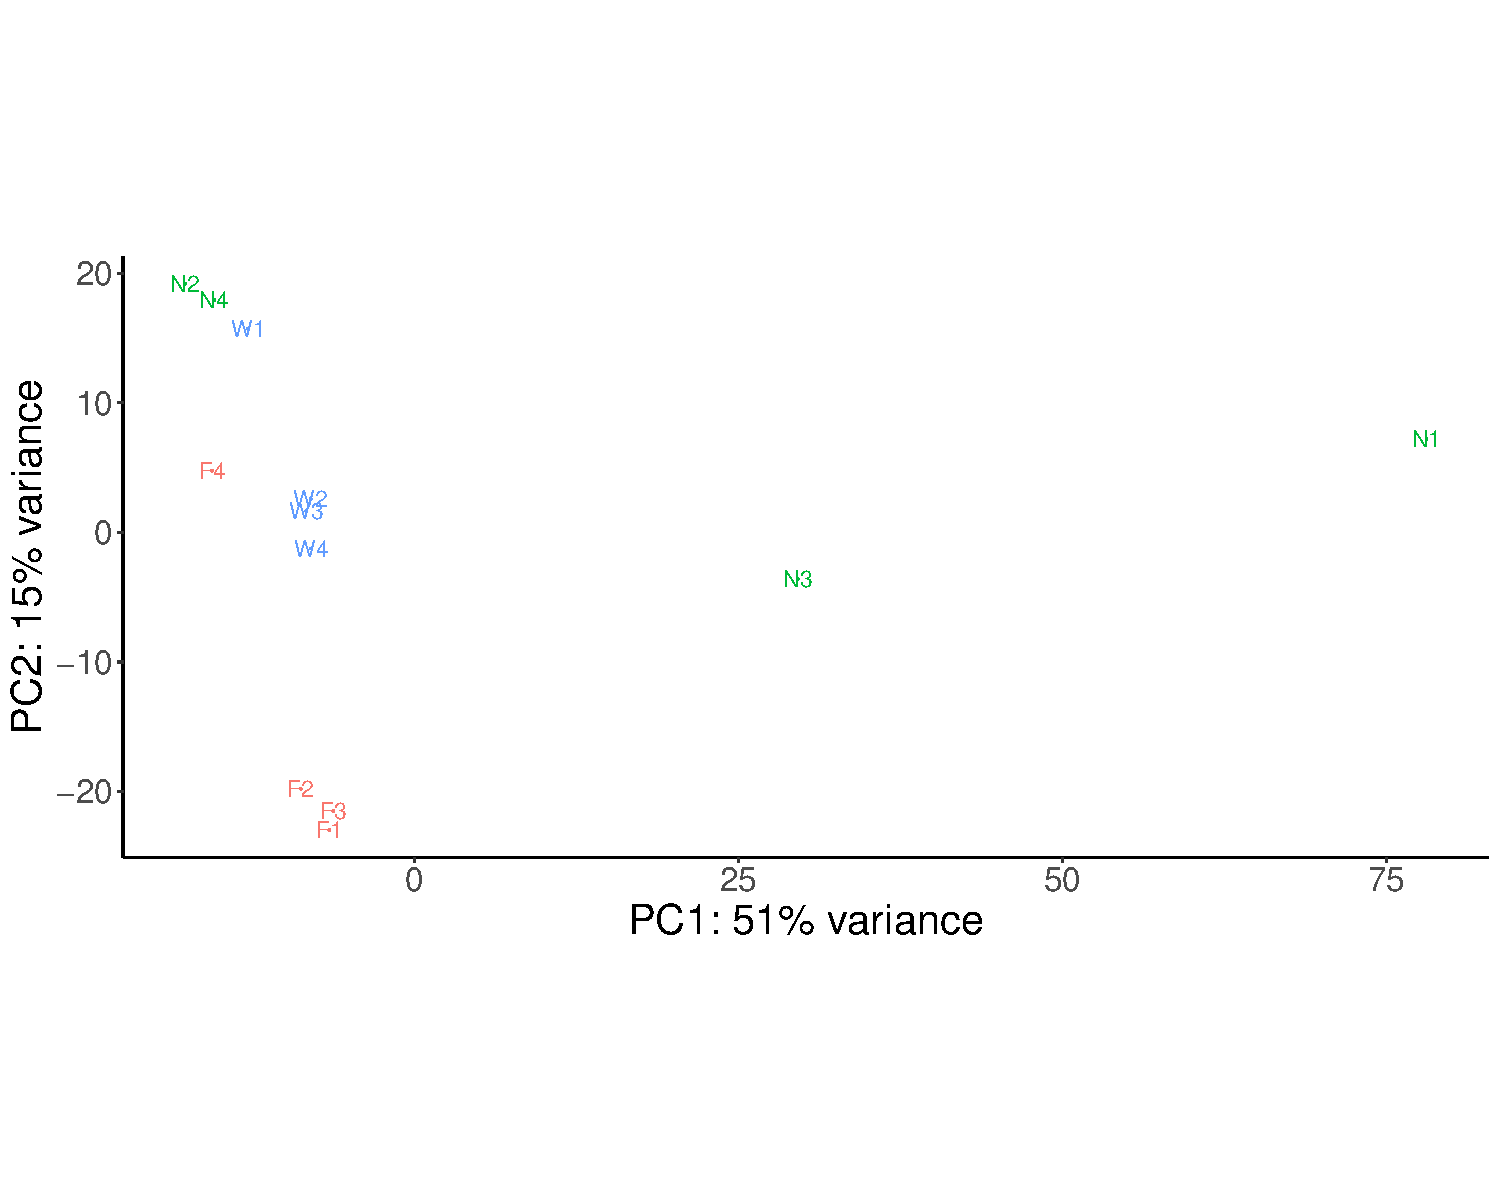
\includegraphics[width=0.75\linewidth]{figs2.pdf} 
    \caption*{\textbf{Figure S2} \quad Fat body tissue sample relationships between nurse, forager, and winter bees as determined by principal component analysis (PCA). Sample relationships determined using all tested genes ($n=9178$).}
    \label{fig:S2}
\end{figure}

\pagebreak

\begin{figure}[ht]
    \centering
		\includegraphics[width=0.75\linewidth]{figs3.pdf} 
    \caption*{\textbf{Figure S3} \quad PCA projection pursuit outlier map of all fat body tissue samples using all tested genes ($n=9178$).}
    \label{fig:S3}
\end{figure}

\pagebreak

\begin{figure}[ht]
    \centering
    \begin{subfigure}[t]{0.45\textwidth}
        \centering
        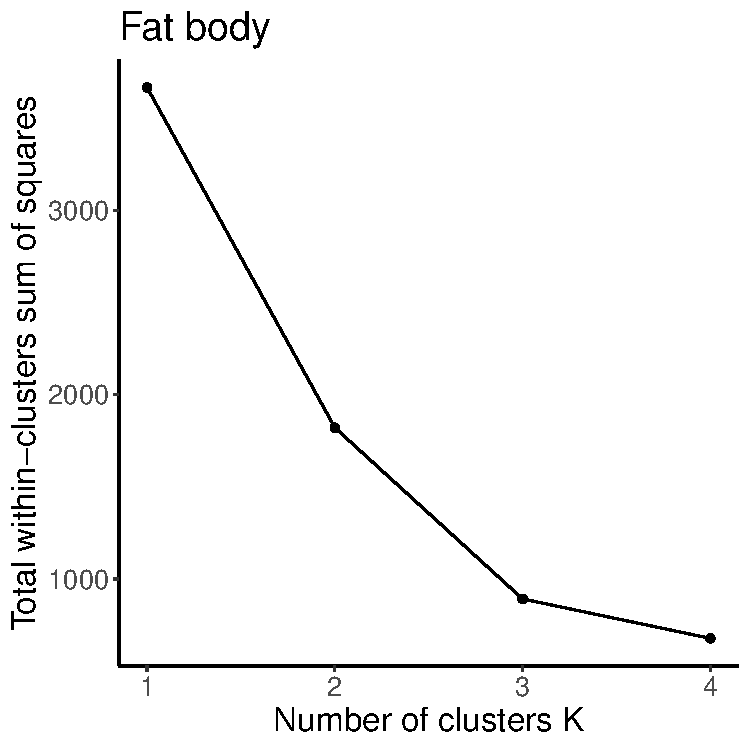
\includegraphics[width=\linewidth]{figs4a.pdf} 
        \caption{Fat body} \label{fig:S4a}
    \end{subfigure}
    \hfill
    \begin{subfigure}[t]{0.45\textwidth}
        \centering
        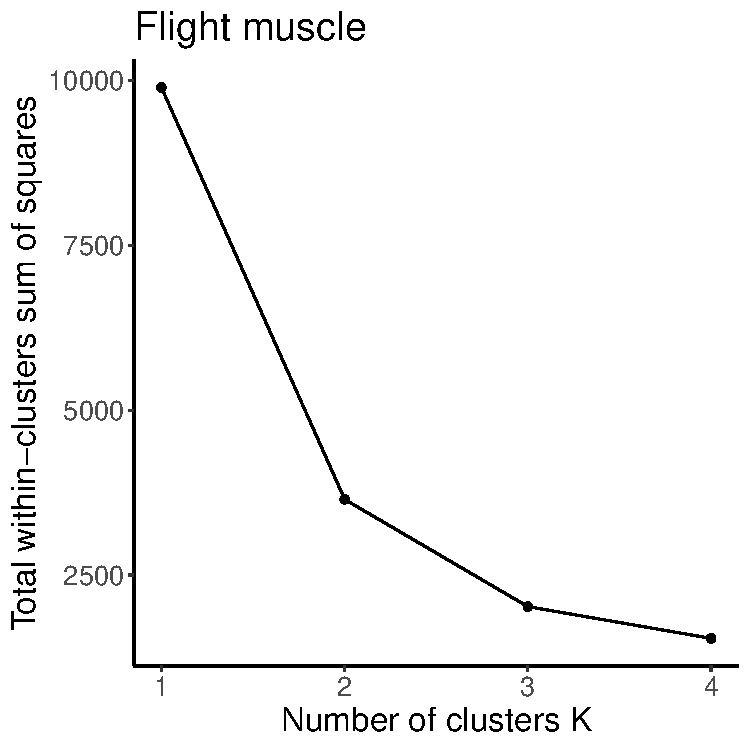
\includegraphics[width=\linewidth]{figs4b.pdf} 
        \caption{Flight muscle} \label{fig:S4b}
    \end{subfigure}
    \caption*{\textbf{Figure S4} \quad Within-cluster variance explained by different values of \textit{k} using all tested genes ($n=9178$).}
\end{figure}

\pagebreak

\begin{figure}[ht]
    \centering
		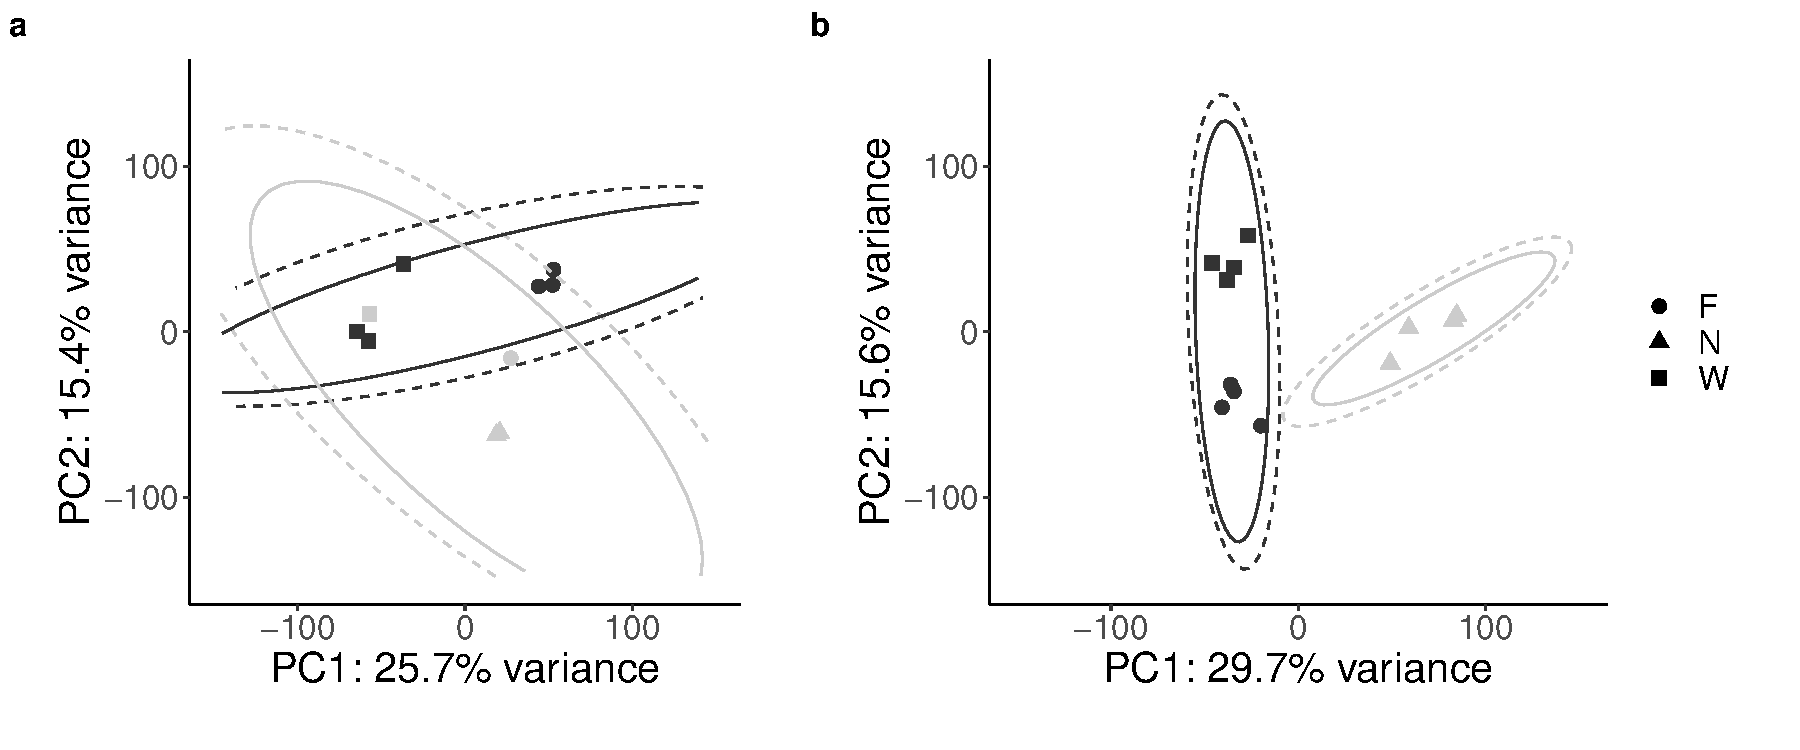
\includegraphics[width=1\linewidth]{figs5.pdf} 
     \caption*{\textbf{Figure S5} \quad k-means clustering of (a) fat body and (b) flight muscle tissue samples using FvN DEGs ($n=1266$). Dotted lines indicate 95\% confidence intervals.}
    \label{fig:S5}
\end{figure}

\end{document}